\documentclass[11pt]{beamer} 

% 
%==> Preamble
%

%
%==> Standard packages
%
\usepackage{hyperref,amsmath,amssymb,mathtools}
\usepackage{hyperref,mathrsfs,enumerate,xcolor,pgfkeys}

%
%==> Theme support
%
\usepackage{helvet}
\definecolor{links}{HTML}{2A1B81}
\hypersetup{colorlinks,linkcolor=,urlcolor=links}
\mode<presentation>{
	\usetheme{Pittsburgh}
	\usecolortheme{seagull}
	}
% Set all frame titles to bold face
\setbeamerfont{frametitle}{series=\bfseries}
% Set default section counter to 0
%\setcounter{section}{-1}

%
%==> Code support
%
\usepackage{listings,algorithm,algorithmic}
\colorlet{verylightgray}{lightgray!50}
\lstset{
	language=bash,
	basicstyle=\ttfamily,
	backgroundcolor=\color{verylightgray},
	mathescape=false
	}


%
%==> Begin document
%
\begin{document}

%
%==> Title page
%

%
%==> Title
%

\title{
	\bf A very brief introduction to git
	}

%
%==> Author
%
\author{
	Jon Tjun Seng Lo Kim Lin \\
	\href{mailto:jlokimlin@math.ucsb.edu}{\tt jlokimlin@math.ucsb.edu}
	}

%
%==> Date
%
\date{
	UCSB Hypatian Seminar\\
	04/25/16
	}

\begin{frame}

	\maketitle

\end{frame}


%
%==> Quote
%
%
%==> quote
%
\begin{frame}

  \begin{center}
    \large You broke the build! - \textbf{Anonymous}
  \end{center}

\end{frame}


%
%==> Outline
%
\begin{frame}
  \frametitle{
    Outline
  }
  \tableofcontents
\end{frame}

%
%===> Section 0: Motivation
%
\section{
  Motivation
}
%
%==> What is the purpose of git?
%
\begin{frame}
	\frametitle{
	What is the purpose of git?
	}
	\begin{itemize}%[<+->]
	\item
          Suppose you're an exemplary grad student, working {\bf VERY} diligently on your research.
        \item
          As you're progressing through your project, it is natural for you to experiment.
        \item
          \textcolor{red}{Then you realize, your experiment/the direction you took went awry.}
        \item
          You reach a point where you say \textcolor{blue}{\bf "D\#@\&\$....why did I not save that earlier version of my project!"}
	\end{itemize}
\end{frame}
%
%==> Git comes to the rescue
%
\begin{frame}[fragile]
	\frametitle{
	Git comes to the rescue
	}
	\begin{itemize}%[<+->]
	\item
          \textcolor{red}{
            No more saving {\tt version1.f90, version2.f90, version3.f90, version4.f90, version5.f90,...} of your code.
          }
        \item
          Git will assist in tracking your revisions. 
	\item
          More formally, Git is a \href{
            http://en.wikipedia.org/wiki/Distributed\_revision\_control}{
            \bf distributed version control (DVC)
          }
          and \href{
            http://en.wikipedia.org/wiki/Revision\_control}{
            \bf source code management (SCM)
          } system.
        \item
          More importantly however, \textcolor{blue}{Git is your new best friend!}
	\end{itemize}
\end{frame}
%
%==> The basics of Git
%
\begin{frame}
  \frametitle{
    \bf The basics of Git
  }
  \begin{enumerate}%[<+->]
  \item
    Where can I get Git?
  \item
    Intro and basic commands
  \item
    Remote repositories
  \item
    Resources
  \end{enumerate}
\end{frame}


%
%==> Section 1: Where can I get Git?
%
%
%==> Section 1: Where can I get Git?
%
\section{
  Where can I get Git?
  }
%
%==> Where can I get Git?
%
\begin{frame}[fragile]
  \frametitle{
    Where can I get Git?
  }

  \textcolor{red}{Installing Git:} You can either install it as a package or via another installer, or download the source code and compile it yourself.

\end{frame}

%
%==> Installing on Mac
%
\begin{frame}[fragile]
  \frametitle{
    Installing on Mac
  }
  \begin{itemize}%[<+->]
  \item
    A Mac OS X Git installer is maintained and available for download at \href{http://git-scm.com/download/mac}{http://git-scm.com/download/mac}, or better yet;
  \item
    \textcolor{red}{Homebrew}, “the missing package manager for OS X,” allows you to easily install hundreds of open-source tools, see: \href{https://brew.sh/}{https://brew.sh/}

    \bigskip

    With Homebrew, installing Git is as easy as this:

    \begin{lstlisting}
      brew update
      brew install git
    \end{lstlisting}
    
  \item
    For more detailed instructions, see: \href{http://kj-prince.com/install-git-mac-osx-homebrew/}{http://kj-prince.com/install-git-mac-osx-homebrew/}.
  \end{itemize}

\end{frame}

%
%==> Installing on Windows
%
\begin{frame}[fragile]
\frametitle{\bf
Installing on Windows
}

Windows:\href{http://msysgit.github.io/}{http://msysgit.github.io/}

\end{frame}

%
%==> Installing on GNU/Linux
%
\begin{frame}[fragile]
  \frametitle{
    Installing on GNU/Linux
  }

Use the \textcolor{blue}{package-manager} that comes with your distribution.

\begin{itemize}%[<+->]
\item
  If you're on a Debian-based distribution like Ubuntu, try {\tt apt-get}:
  \begin{lstlisting}
    $ sudo apt-get install git
  \end{lstlisting}
\item
  If you're on Fedora for instance, try {\tt yum}:
  \begin{lstlisting}
    $ sudo yum install git-all
  \end{lstlisting}
\end{itemize}

For different Unix-like flavors, see: \href{http://git-scm.com/download/linux}{http://git-scm.com/download/linux}.

\end{frame}


%
%==> Section 2: Intro and basic commands
%
%
%==> Intro and basic commands
%
\section{Intro and basic commands}

%
%==> Basic commands
%
\begin{frame}[fragile]
  \frametitle{
    Basic commands
  }

  \begin{itemize}%[<+->]
  \item
    {\tt git init} - initializes a Git repository.
  \item
    {\tt git add} - adds files to your repository.
  \item
    {\tt git commit} - creates a commit. Commits allow Git to keep track of your revisions, similar to saving files.
  \item
    {\tt git status} - shows the status of your Git repository (i.e. what files have been changed, what files are not accounted for, etc).
  \end{itemize}

\end{frame}

%
%==> The basic git workflow is:
%
\begin{frame}
  \frametitle{
    The basic Git workflow is
  }

  \begin{itemize}%[<+->]
  \item
    \textcolor{blue}{\bf modify files} in your working directory.
  \item
    \textcolor{blue}{\bf stage files} you've worked on. This prepares a snapshot of the directory
  \item
    \textcolor{blue}{\bf commit the files} you've staged. This stores that snapshot in the git repository.
  \end{itemize}

\end{frame}

%
%==> Initializing repositories
%
\begin{frame}[fragile]
  \frametitle{
    Initializing repositories
  }

  To initialize a new project, in the project directory, initialize the git repository with:

  \begin{lstlisting}
    git init
  \end{lstlisting}

  %Remark: This will enable git to keep track of changes in this folder, and subfolders by creating a {\tt .git} hidden folder containing the git skeleton.

  The second way is:

  \begin{lstlisting}
    git clone https://github.com/jlokimlin
    /intro\_to\_git.git
  \end{lstlisting}

  %Remark: This will clone an existing repository into your currect directory.

  \textcolor{red}{
    {\bf Warning:} Each new repository should be in its own directory. One git repository should {\bf not} be created or cloned in an {\bf existing git repository}, i.e., a folder you've initialized a git repository and its subfolders.
  }

\end{frame}

%
%==> Configuring Git
%
\begin{frame}[fragile]
  \frametitle{
    Configuring Git
  }

  You will have to do this \textcolor{red}{\bf once} per computer you use {\tt git config --global:}

  {
    \footnotesize
    \begin{lstlisting}
      git config --global user.name "Your Avatar"
      git config --global user.email you@domain.com''
      git config --global core.editor vim
      git config color.ui auto
    \end{lstlisting}
  }
  
% Remark: The {\tt --global} option corresponds to a user-wide configuration. The configuration will be stored in a hidden repository in your home. You can also configure each git repository individually, by removing this option, or system-wide by replacing the {\tt --global} option with {\tt --system}. Usually, we just configure repositories user-wide.

  You can check your configuration with:
  \begin{lstlisting}
    git config --list
  \end{lstlisting}

  % Remark: If you've configured git several times at different levels, you will probably see several entries twice or three times in the configuration list. The user-wide configuration overrides the system-wide configuration, and the local configuration overrides the user-wide configuration.

\end{frame}

%
%==> Working locally
%
\begin{frame}[fragile]
  \frametitle{
    Working locally
}

  % Remark: One of the main goal of version control is to save snapshots of your directory. We call those snapshots commits. To each snapshot is associated some metadata: the date the snapshot was taken, who took it, what files where modified, the changes that were made on those files etc. Git will enable you to track the changes made to the files, revert the entire project to a previous snapshot, review changes made over time, view who modified a file. Now that we know why we want to create a snapshot, let's see how to do this.

  Right now, nothing in the project is tracked. First let's create some directories and files in our directory.

  \begin{lstlisting}
    touch README.md
  \end{lstlisting}

  First, you need to tell git this file exists:

  \begin{lstlisting}
    git add README.md
  \end{lstlisting}

  Now you can commit it:

  \begin{lstlisting}
    git commit -m "Added a README file"
  \end{lstlisting}

  At this point, you have one tracked file, and an initial commit. 

\end{frame}

%
%==> File status lifecycle
%
\begin{frame}[fragile]

  % Remark: Each file in the working directory can be in one of two states: tracked or untracked. Any file you have not explicitly added at some point is untracked. Tracked files can themselves be in different states: unmodified, modified or staged.
  
  \begin{center}
    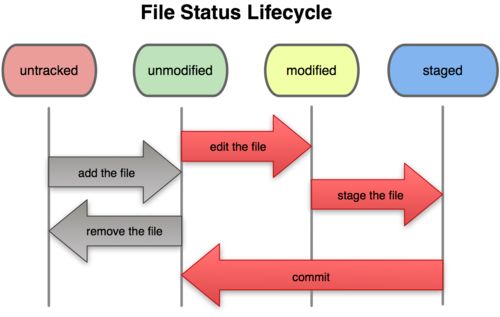
\includegraphics[scale=1.25]{./graphics/git_file_status_lifecycle.png}
  \end{center}

\end{frame}

%
%==> The git status command
%
\begin{frame}[fragile]
  \frametitle{
    The git status command
  }

  The {\tt git status} command will display all untracked files, and modified and staged files in your directory:

  \begin{lstlisting}
    touch AUTHORS.txt
    git status
  \end{lstlisting}

  Now, try
  \begin{lstlisting}
    git add AUTHORS.txt
    git status
  \end{lstlisting}

  {\tt git add} is also used to stage file. In fact, running {\tt git add} on an untracked file not only tracks it, but stages it.

  \begin{lstlisting}
    git commit -m "Added the AUTHORS file"
  \end{lstlisting}

  And here is the second commit! 

\end{frame}
%
%==> Tracking changes to a modified file
%
\begin{frame}[fragile]
  \frametitle{
    Tracking changes to a modified file
  }

  Sometimes, you may want to look at the changes you've made to a modified file:

  \begin{lstlisting}
    git diff
  \end{lstlisting}

  To look at the changes you've made in the staged files, simply use:

  \begin{lstlisting}
    git diff --cached
  \end{lstlisting}

  And to view the history of all commits:

  \begin{lstlisting}
    git log
  \end{lstlisting}

\end{frame}

%
%==> (Re)moving files
%
\begin{frame}[fragile]
  \frametitle{
    (Re)moving files
  }

  \begin{itemize}
  \item
    \textcolor{red}{Deleting files:} Why use {\tt git rm} to remove a file instead of {\tt rm}?
    \begin{itemize}
    \item
      If you just use {\tt rm}, you will need to follow it up with {\tt git add <fileRemoved>} The command {\tt  git rm} does both in one step.
    \item
      You can also use {\tt git rm --cached} which will remove the file from the index (staging it for deletion on the next commit), but keep your copy in the local file system.
      \end{itemize}
  \item
    \textcolor{red}{Moving files:} In a similar fashion, {\tt git mv} can be used to move a file in one step.
  \end{itemize}

\end{frame}

%
%==> Canceling stages
%
\begin{frame}[fragile]
  \frametitle{
    Canceling stages
  }
  
  %Remark: Because to err is human, you may want to cancel some stages.
  Two scenarios may occur:
  \begin{enumerate}
  \item
    \textcolor{blue}{you staged a file you do not want to commit}
  \item
    \textcolor{red}{you made some changes on a file you want to cancel.}
  \end{enumerate}

  First, let's assume you've staged a file you want to unstage:

  \begin{lstlisting}
    touch myFile.tex
    git add myFile.tex
  \end{lstlisting}

  To unstage it, run:

  \begin{lstlisting}
    git reset HEAD myFile.tex
  \end{lstlisting}

  %Remark: The syntax is git reset HEAD <filename>. We will explain what HEAD is later on.
  Second, say you've modified a file and you want to cancel the changes.
  \begin{lstlisting}
    git checkout myFile.tex
  \end{lstlisting}

  %Remark: If you run {\tt git status}, you can notice git reminds you what command to use for which action.
  
\end{frame}


%
%==> Section 3:  Remote repositories
%
%
%==> Section 3: Remote repositories
%
\section{
  Remote repositories
}

%
%==> Main competitors
%
\begin{frame}
  \frametitle{
    Remote repositories - Main competitors
  }

  \begin{itemize}%[<+->]
  \item
    GitHub: \href{https://github.com/}{https://github.com/}
  \item
    Bitbucket: \href{https://bitbucket.org/}{https://bitbucket.org/}
  \end{itemize}
\end{frame}

%
%==>  Create your own remote repository
%
\begin{frame}[fragile]
  \frametitle{
    Create your own remote repository
  }

  Create your own repository on \textcolor{red}{GitHub (\$7 a month for private repo's)} or \textcolor{blue}{Bitbucket (free unlimited private repo's)}.

  \bigskip  

  This can be for an existing or a new project.

  \bigskip
  
  {\bf More commands:}
  \begin{itemize}
  \item
    {\tt git clone} - imports a remote repository.
  \item
    {\tt git pull} - extracts most recent changes from a repository.
  \item
    {\tt git push} - broadcast your changes to a repository.
  \end{itemize}

\end{frame}

%
%==>  A distant repository with GitHub
%
\begin{frame}[fragile]
  \frametitle{
    A distant repository with GitHub
  }

  % Remark: Up to now, we've been working locally on our computer. As a scientist, you may want to share your work, (or better contribute to an opensource project!). This is where Bitbucket comes in handy. Bitbucket is a web hosting platform for git projects. Not only does it provide free git repository for opensource projects (private repo's are free for up to 5 group users), but it provides great tools to review code, manage projects, release packages and publish documentation.
  
% Now, let's go on Bitbucket, and create an account. Once this is done, We can easily create a new project by clicking on the create button, on the main page.

  \begin{center}
    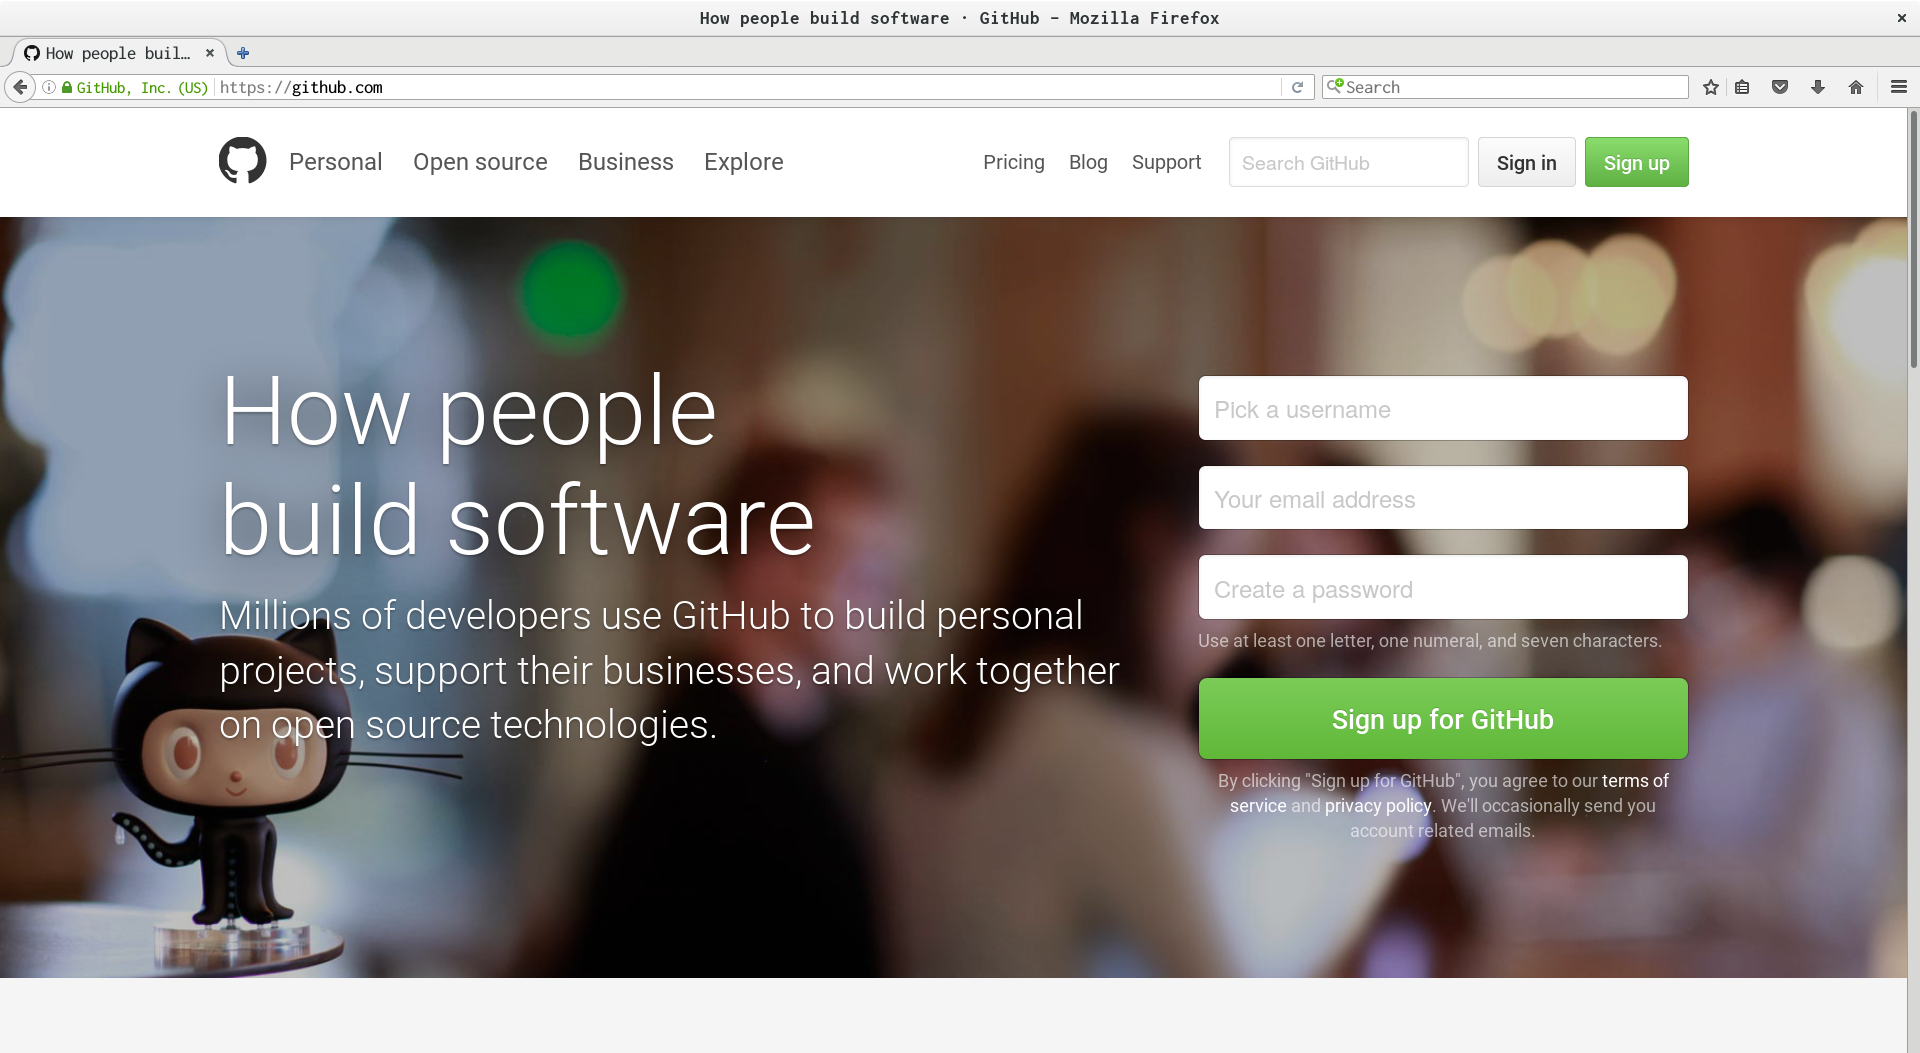
\includegraphics[scale=0.155]{./graphics/github_homepage.png}
  \end{center}

\end{frame}
%
%==> GitHub profile
%
\begin{frame}[fragile]
  \frametitle{
   GitHub profile
  }

  \begin{center}
    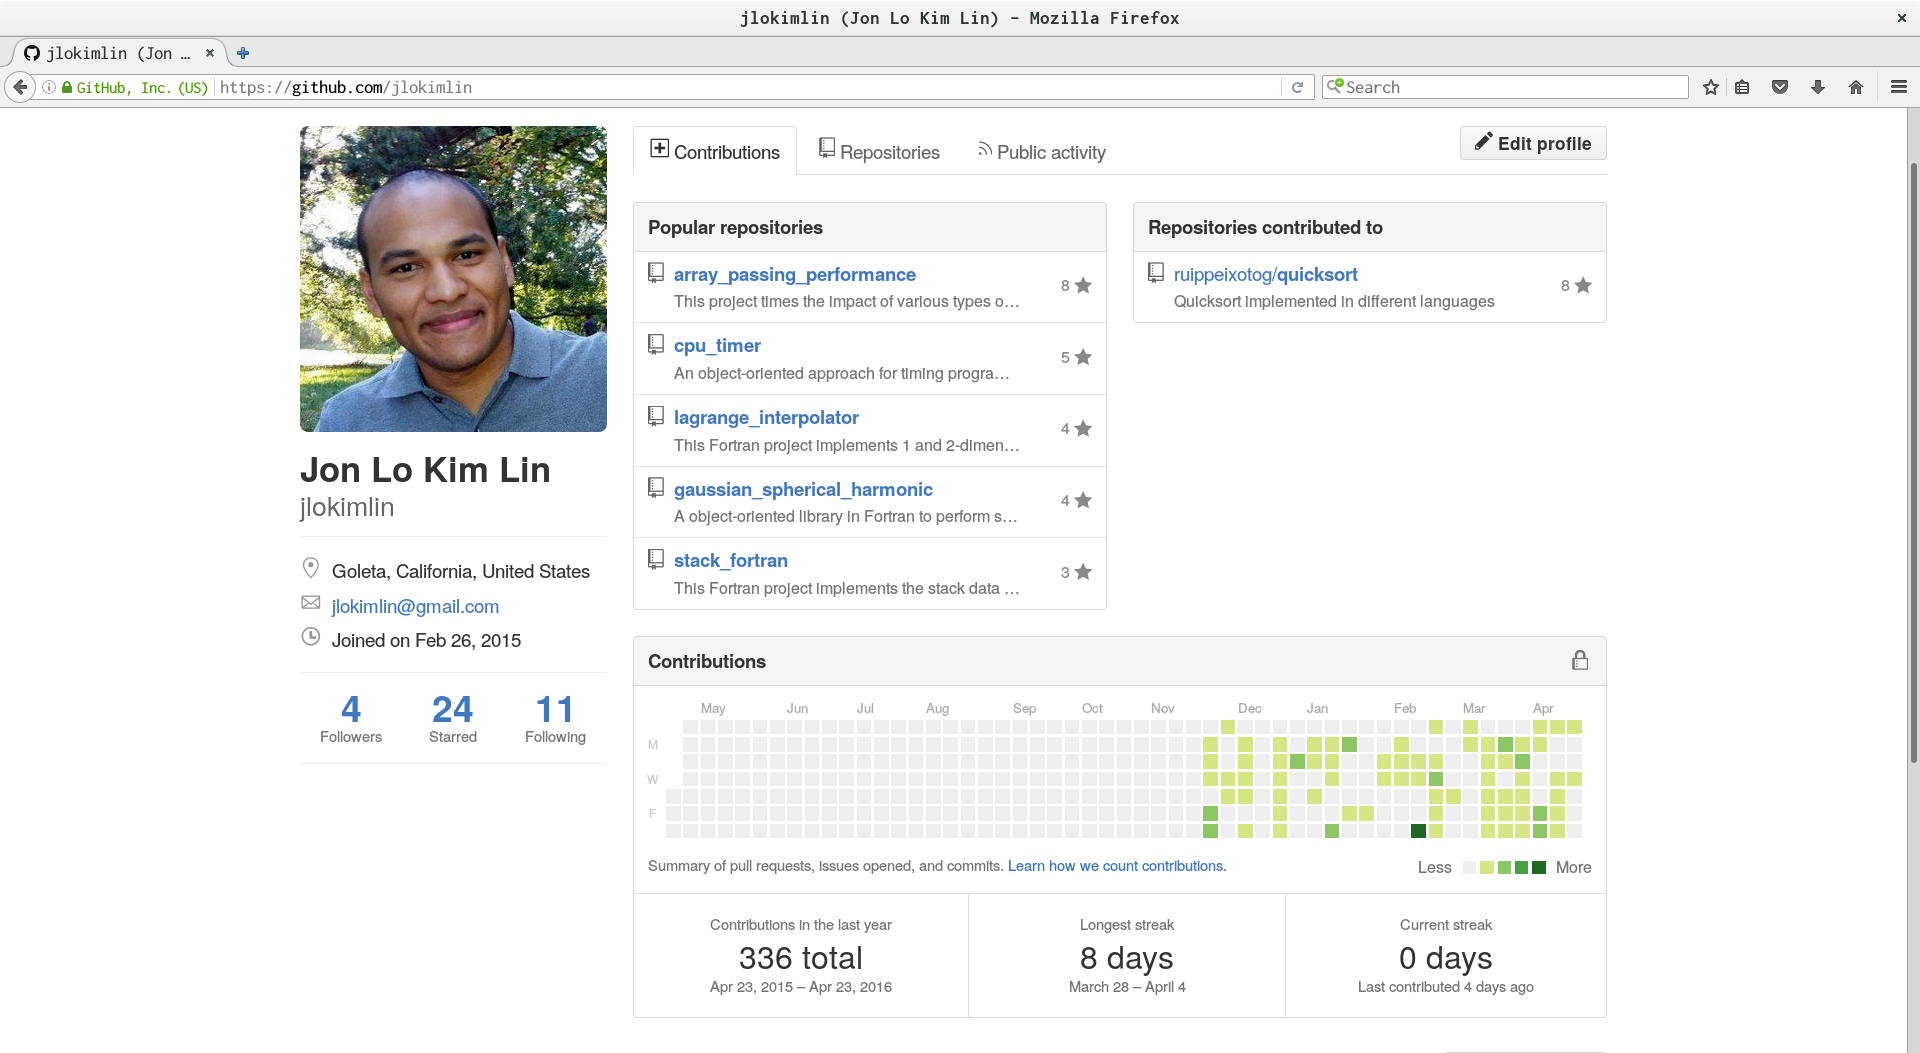
\includegraphics[scale=0.155]{./graphics/jlokimlin_github_profile.png}
  \end{center}

\end{frame}
%
%==> Create new repository
%
\begin{frame}[fragile]
  \frametitle{
    Create new repository
  }

  \begin{center}
    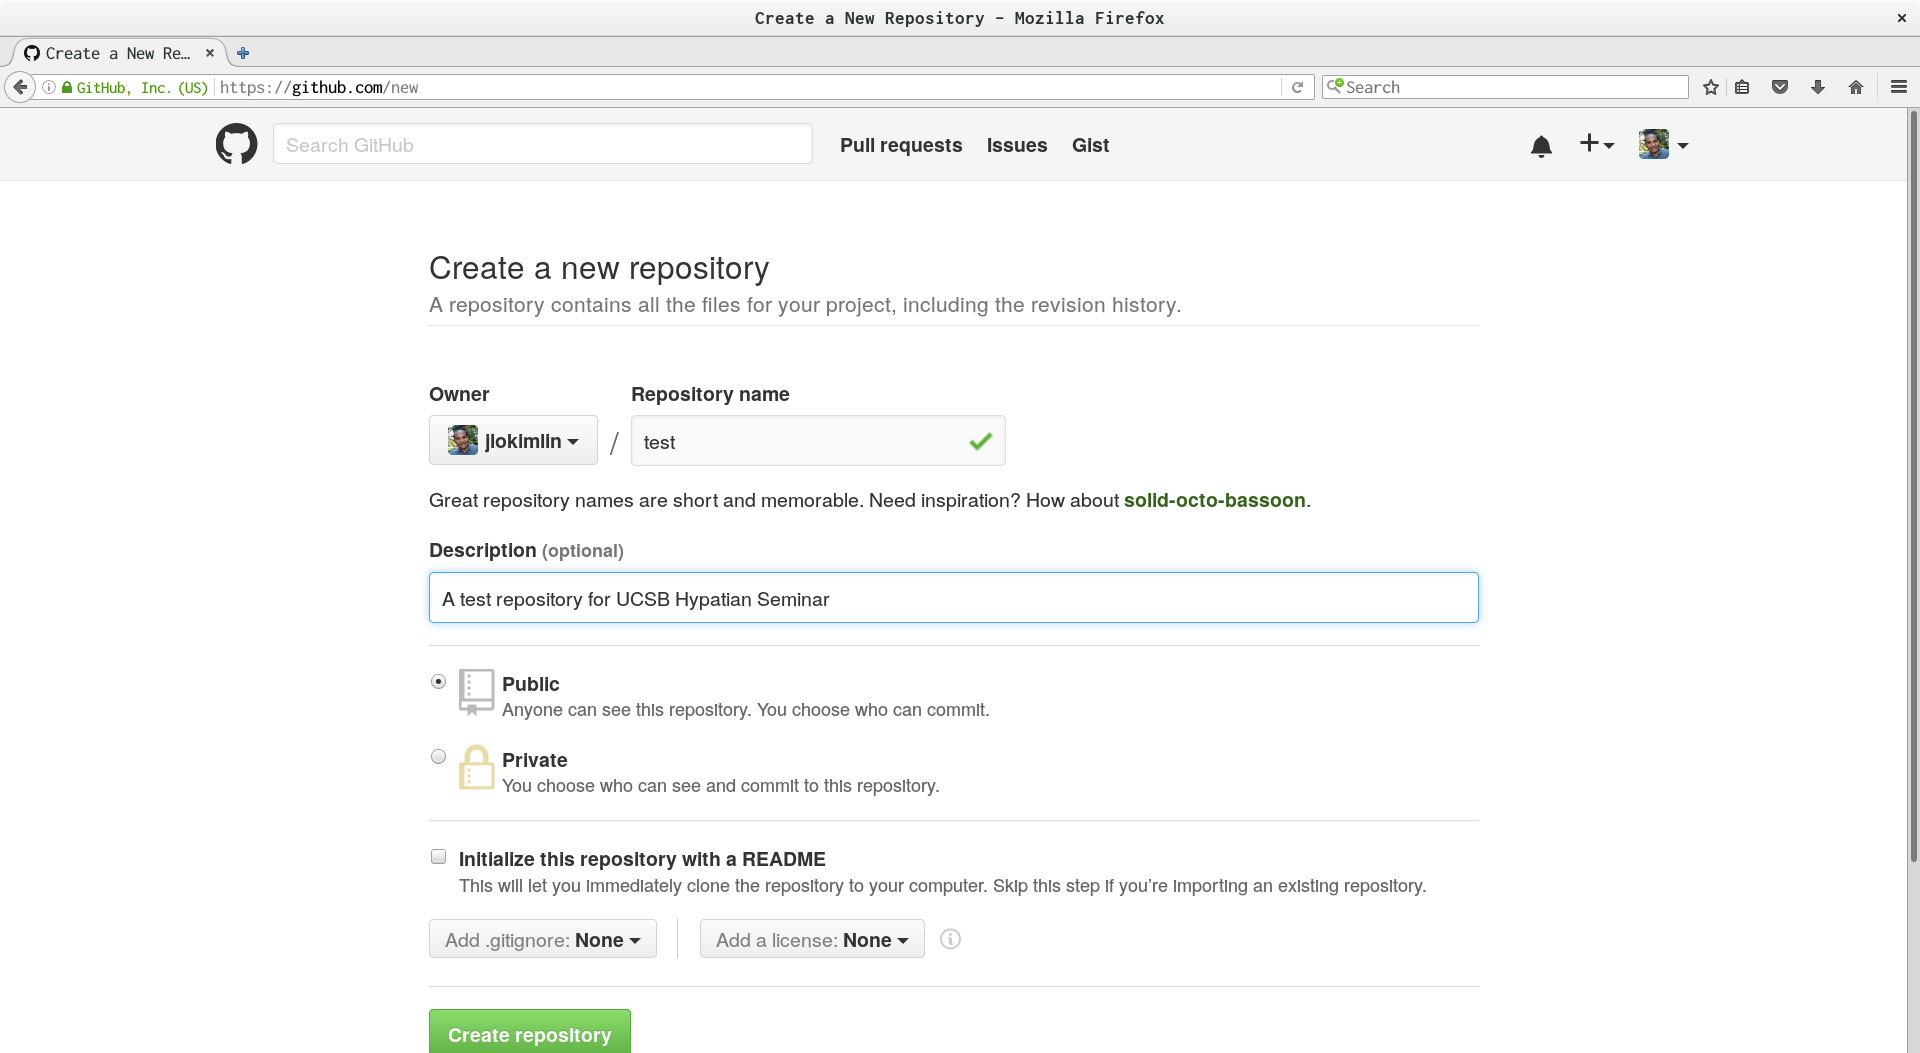
\includegraphics[scale=0.155]{./graphics/create_new_repository.png}
  \end{center}

\end{frame}

%
%==> A distant repository with Bitbucket (continued)
%
\begin{frame}[fragile]
  \frametitle{
    Create a new repository (continued)
  }
  
  \begin{center}
    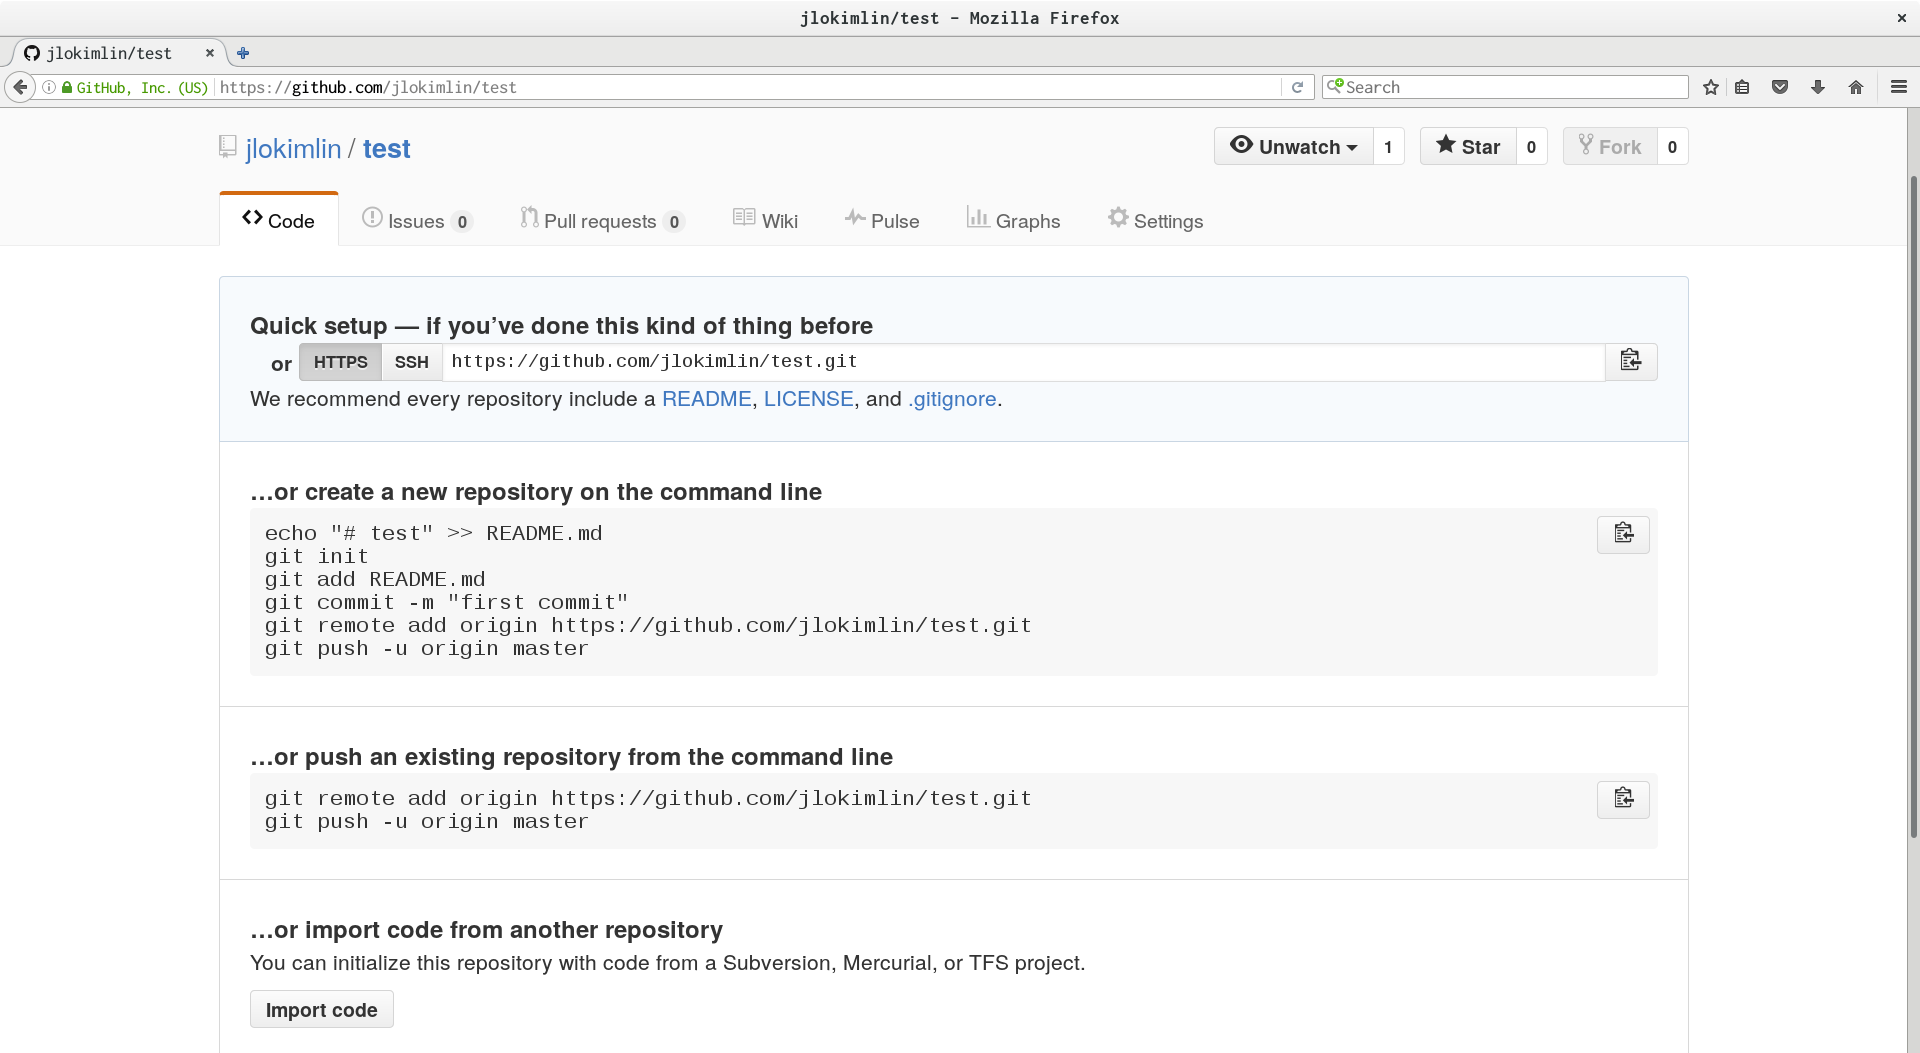
\includegraphics[scale=0.15]{./graphics/new_repo_continued.png}
  \end{center}

\end{frame}

%
%==> Create a new repository on the command line
%
\begin{frame}[fragile]
  \frametitle{
    Create a new repository on the command line
  }

  \begin{lstlisting}
    mkdir /path/to/your/project
    cd /path/to/your/project
    echo "# test" >> README.md
    git init
    git add README.md
    git commit -m "first commit"
    git remote add origin
    https://github.com/jlokimlin/test.git
    git push -u origin master
  \end{lstlisting}
\end{frame}

%
%==> Push an existing repository from the command line
%
\begin{frame}[fragile]
  \frametitle{
    Push an existing repository from the command line
  }

  \begin{lstlisting}
    mkdir /path/to/your/project
    cd /path/to/your/project
    git remote add origin
    https://github.com/jlokimlin/test.git
    git push -u origin master
  \end{lstlisting}

\end{frame}


%
%==> Section 4: Resources
%
%
%==> Section 4: Resources
%
\section{
  Resources
}

\begin{frame}
  \frametitle{
    Resources
  }

  \begin{itemize}%[<+->]
  \item
    A personal favorite on Bitbucket for git:
    \href{https://www.youtube.com/watch?v=BtEvnE79jxY}{https://www.youtube.com/watch?v=BtEvnE79jxY}
  \item
    Everyday git with 20 commands:\\
    \href{https://www.kernel.org/pub/software/scm/git/docs/everyday.html}{https://www.kernel.org/pub/software/scm/git\\/docs/everyday.html}
  \item
    Git tutorial:\\
    \href{https://www.kernel.org/pub/software/scm/git/docs/gittutorial.html}{https://www.kernel.org/pub/software/scm/git\\/docs/gittutorial.html}
  \item
    The (overwhelming) Git manual page:\\
    \href{https://www.kernel.org/pub/software/scm/git/docs/}{https://www.kernel.org/pub/software/scm/git/docs/}
  \end{itemize}

\end{frame}


%
%==> Thank you for your time
%
\begin{frame}

  \begin{center}
    {
      \huge \bf Thank you for your time
    }
  \end{center}

\end{frame}

%
%===> End document
%
\end{document}
